\documentclass[10pt]{article}

\usepackage{spheric}
%%%TITLE
\title{Particle Trajectory Calculation in SPH}
\date{}

%%AFFILIATIONS
\author[1]{Jiayuan SHEN$^\dagger$}
\author[1]{Wenhuan LU}
\author[2]{Darcy Q. HOU}
\author[3]{Arris S. TIJSSELING}
\affil[1]{School of Computer Software, Tianjin University, China}
\affil[2]{School of Computer Science and Technology, Tianjin University, China}
\affil[3]{Department of Mathematics and Computer Science, Eindhoven University of Technology}

\affil[$\relax$]{\email{\dagger}{shenjiayuan@tju.edu.cn}}


%%DOCUMENT
\begin{document}

\maketitle

%\SelectedTopics{}

%%PLEASE PUT YOUR ABSTRACT HERE
\begin{abstract}
Smoothed particle hydrodynamics (SPH) method is a Lagrangian meshless approach for modelling fluid dynamics problems \cite{liu2003smoothed,violeau2012fluid}. Due to the Lagrangian property, particles change their positions at every time step and hence the calculation of particle trajectories plays an important role in SPH and may largely affect the overall accuracy. Many explicit time integration algorithms have been used in SPH, but the effect of these timestepping schemes on the calculation of particle trajectories has not been well studied. With specially designed 1D and 2D examples, this paper compares the performance of six commonly used timestepping schemes for particle trajectory calculation, including the Euler forward method, modified Euler, second-order Runge-Kutta (RK2), fourth-order Runge-Kutta (RK4), velocity Verlet and leap-frog. Numerical analysis indicates that for problems with (nearly) uniform velocity fields, all schemes can give solutions with adequate accuracy, but the Euler method, modified Euler and RK2 may not predict accurate particle trajectories in certain highly non-uniform velocity fields (see Fig. \ref{fig:52}b-d). These methods may also introduce varying degrees of artificial dispersion that could lead to overestimation of spill area of particle clouds. On the other hand, the algorithms of RK4, velocity Verlet and leap frog can accurately calculate the particle trajectories without artificial dispersion (see Fig. \ref{fig:52}e-f). In order to find the most efficient scheme with acceptable accuracy and cost, the computational costs of these schemes have also been compared.


\begin{figure}[!htb]
\centering
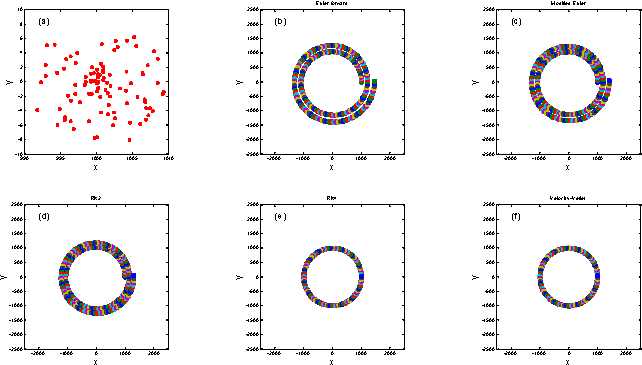
\includegraphics[width=0.85\textwidth]{50-2.pdf}
\caption{Trajectories of (a) 100 random particles calculated by (b) Euler forward, (c) modified Euler, (d) RK2, (e)
RK4 and (f) velocity Verlet.}\label{fig:52}
\end{figure}

\end{abstract}


%%THE END OF ABSTRACT

\addbib

\end{document}
